\documentclass[9pt, handout]{beamer}
\usetheme{CambridgeUS}
\usepackage{xcolor}
\usepackage{geometry}
\usepackage{array}
\usepackage{comment}
\usepackage[export]{adjustbox}

\AtBeginSection[]
{
  \begin{frame}
    \frametitle{Table of Contents}
    \tableofcontents[currentsection]
  \end{frame}
}

\setbeamertemplate{footline}
{
  \leavevmode%
  \hbox{%
    \begin{beamercolorbox}[wd=.333333\paperwidth,ht=2.25ex,dp=1ex,center]{author in head/foot}%
      \usebeamerfont{author in head/foot}\insertshortauthor
    \end{beamercolorbox}%
    \begin{beamercolorbox}[wd=.333333\paperwidth,ht=2.25ex,dp=1ex,center]{title in head/foot}%
      \usebeamerfont{title in head/foot}\insertshortsubtitle
    \end{beamercolorbox}%
    \begin{beamercolorbox}[wd=.333333\paperwidth,ht=2.25ex,dp=1ex,right]{date in head/foot}%
      \usebeamerfont{date in head/foot}\insertshortdate{}\hspace*{2em}
      \usebeamertemplate{page number in head/foot}\hspace*{2ex}
    \end{beamercolorbox}
  }%
  \vskip0pt%
}

\title{Principles of Economics}
\subtitle{Discussion Session 7: Consumer Choice}
\author{Joe Wilske and Yuzhi Yao}
\institute{Boston College}
\date{\today}

\begin{document}

\frame{\titlepage}

\begin{frame}{The Budget Constraint}
    Describes all combinations of $Q_A$ and $Q_B$ that are within your budget.
    \begin{figure}
        \centering
        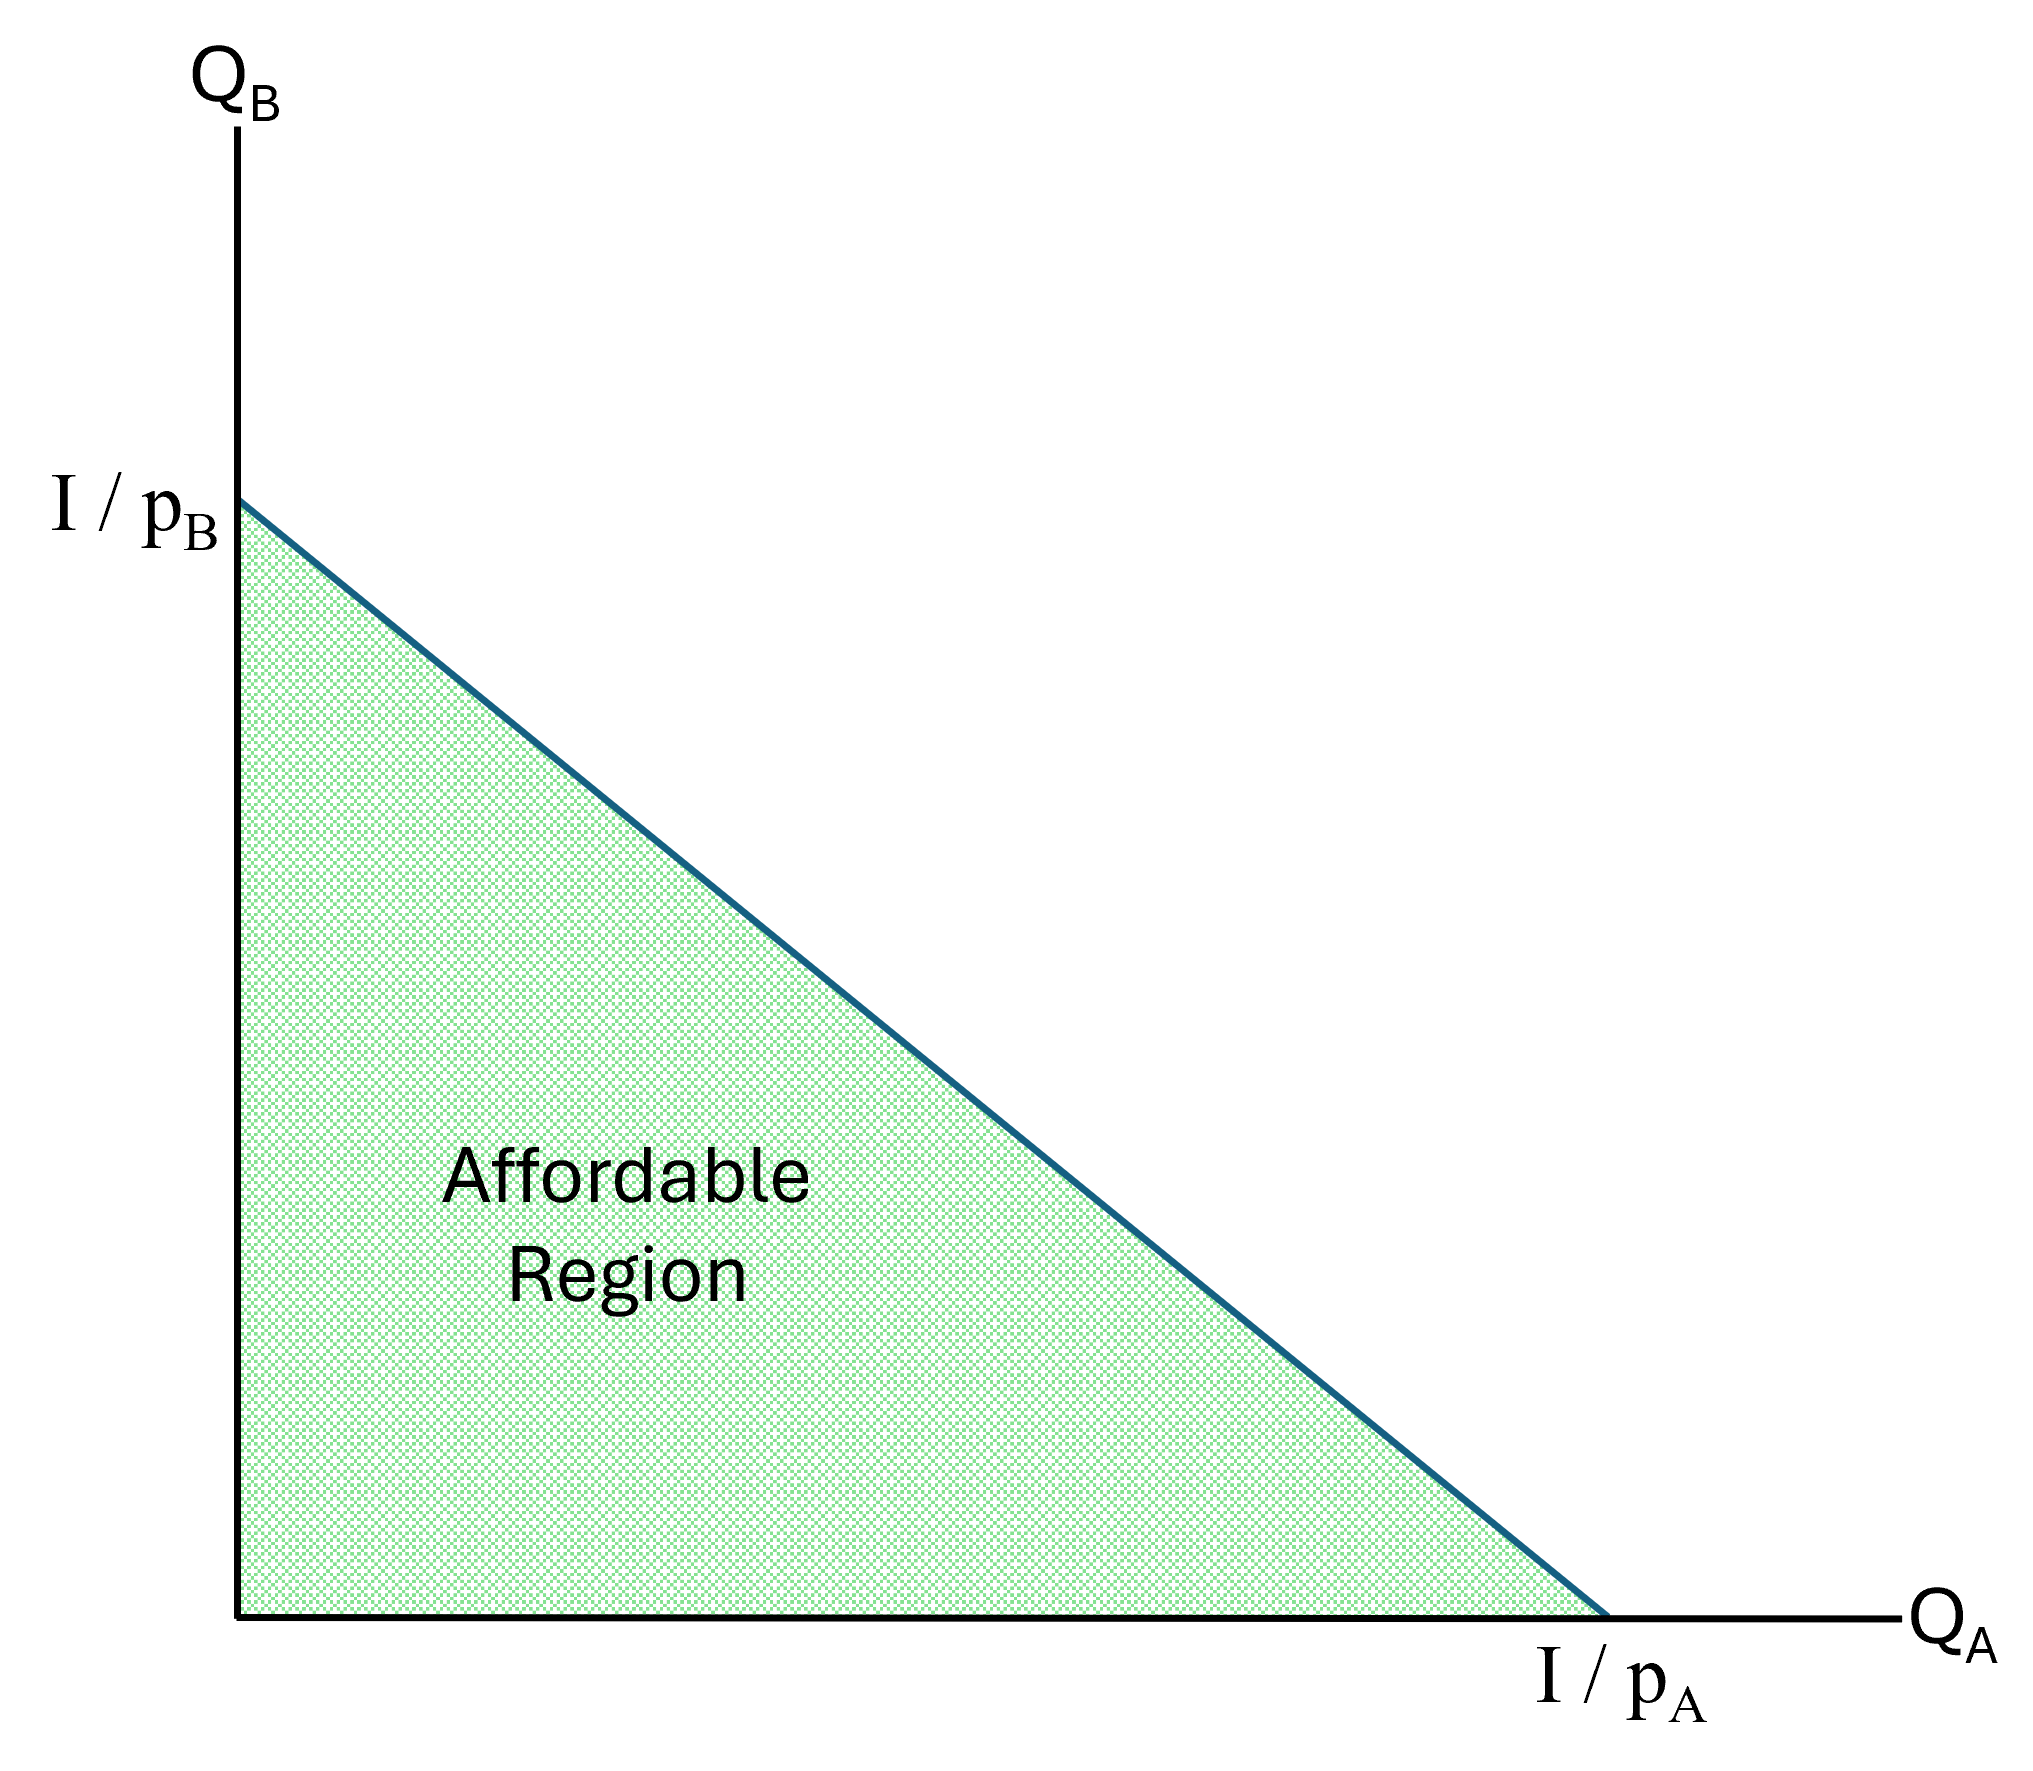
\includegraphics[width=0.65\linewidth]{budget_region.png}
    \end{figure}
\end{frame}

\begin{frame}{Exercise 1: Budget Constraint}
    Q1: Consider two goods, A and B, with $P_A=\$1$ and $P_B=\$2$. Suppose income is \$100. 
    \vspace{7pt}
    \begin{enumerate}
        \item Draw the budget constraint and label the intercepts.
        \vspace{7pt}
        \item How will the budget constraint be affected if 
        \vspace{5pt}
        \begin{itemize}
            \item[-] $P_A$ increases to \$4?
            \vspace{5pt}
            \item[-] Income increases to \$120? (and $P_A$ goes back to \$1)
        \end{itemize}
    \end{enumerate}
    \vspace{1.5in}
\end{frame}

\begin{frame}{Exercise 1: Budget Constraint}
    Solution: 
    \begin{figure}
        \centering
        \includegraphics[width=0.9\linewidth]{sol1.png}
    \end{figure}
\end{frame}

\begin{frame}{Utility Function}
\begin{itemize}
    \item Describes the satisfaction or ``utility" that one receives from consuming a good
    \item Concave $\implies$ diminishing marginal utility
\end{itemize}
    \begin{figure}
        \centering
        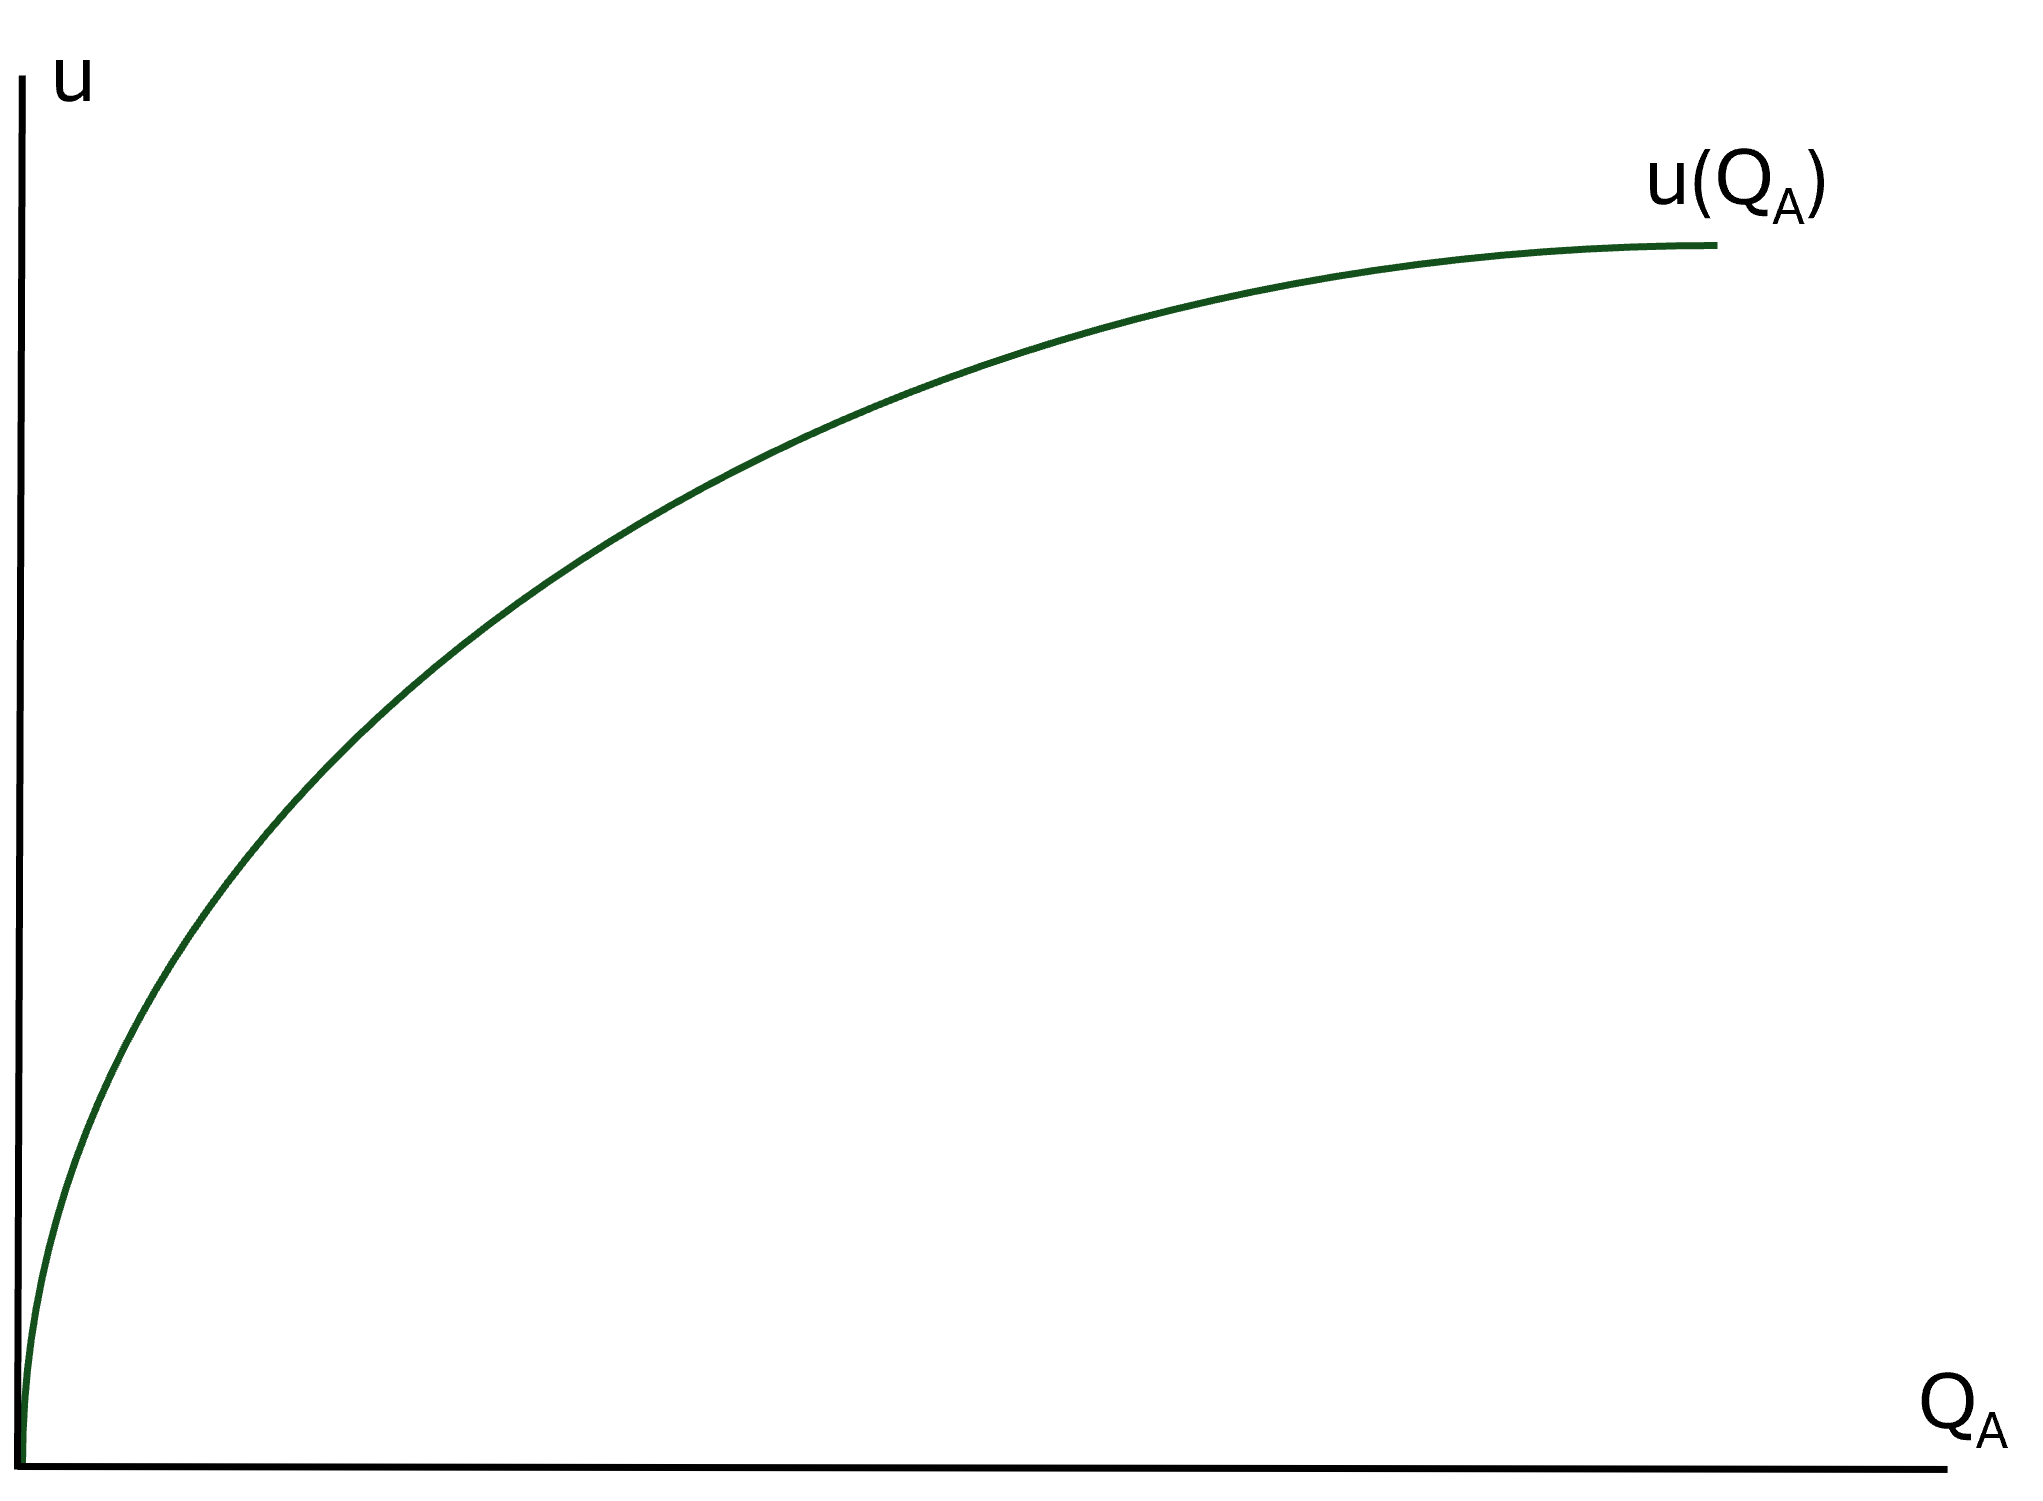
\includegraphics[width=0.5\linewidth]{utility_function.png}
    \end{figure}
    \begin{itemize}
        \item But what if we want to compare the utility from both goods $A$ and $B$?
    \end{itemize}
\end{frame}

\begin{frame}{Utility in 3 Dimensions}
\begin{columns}[c]
\begin{column}{0.5\textwidth}
\begin{itemize}
    \item Add another axis!\\
    $\implies$ Utility depends on $Q_A$ and $Q_B$
    \vspace{5pt}
    \item Can translate this to 2D by depicting curves where utility is constant
    \vspace{5pt}
    \begin{itemize}
        \item Like a topographical map
    \end{itemize}
\end{itemize}
\end{column}
\begin{column}{0.5\textwidth}
    \includegraphics[width=\linewidth]{utility1.png}
    \end{column}
\end{columns}
\end{frame}

\begin{frame}{Indifference Curves}
    \begin{itemize}
        \item Every combination of $A$ and $B$ along the same curve gives the same utility
        \item The consumer is ``indifferent" between all points on the same curve
    \end{itemize}
    \begin{figure}
        \centering
        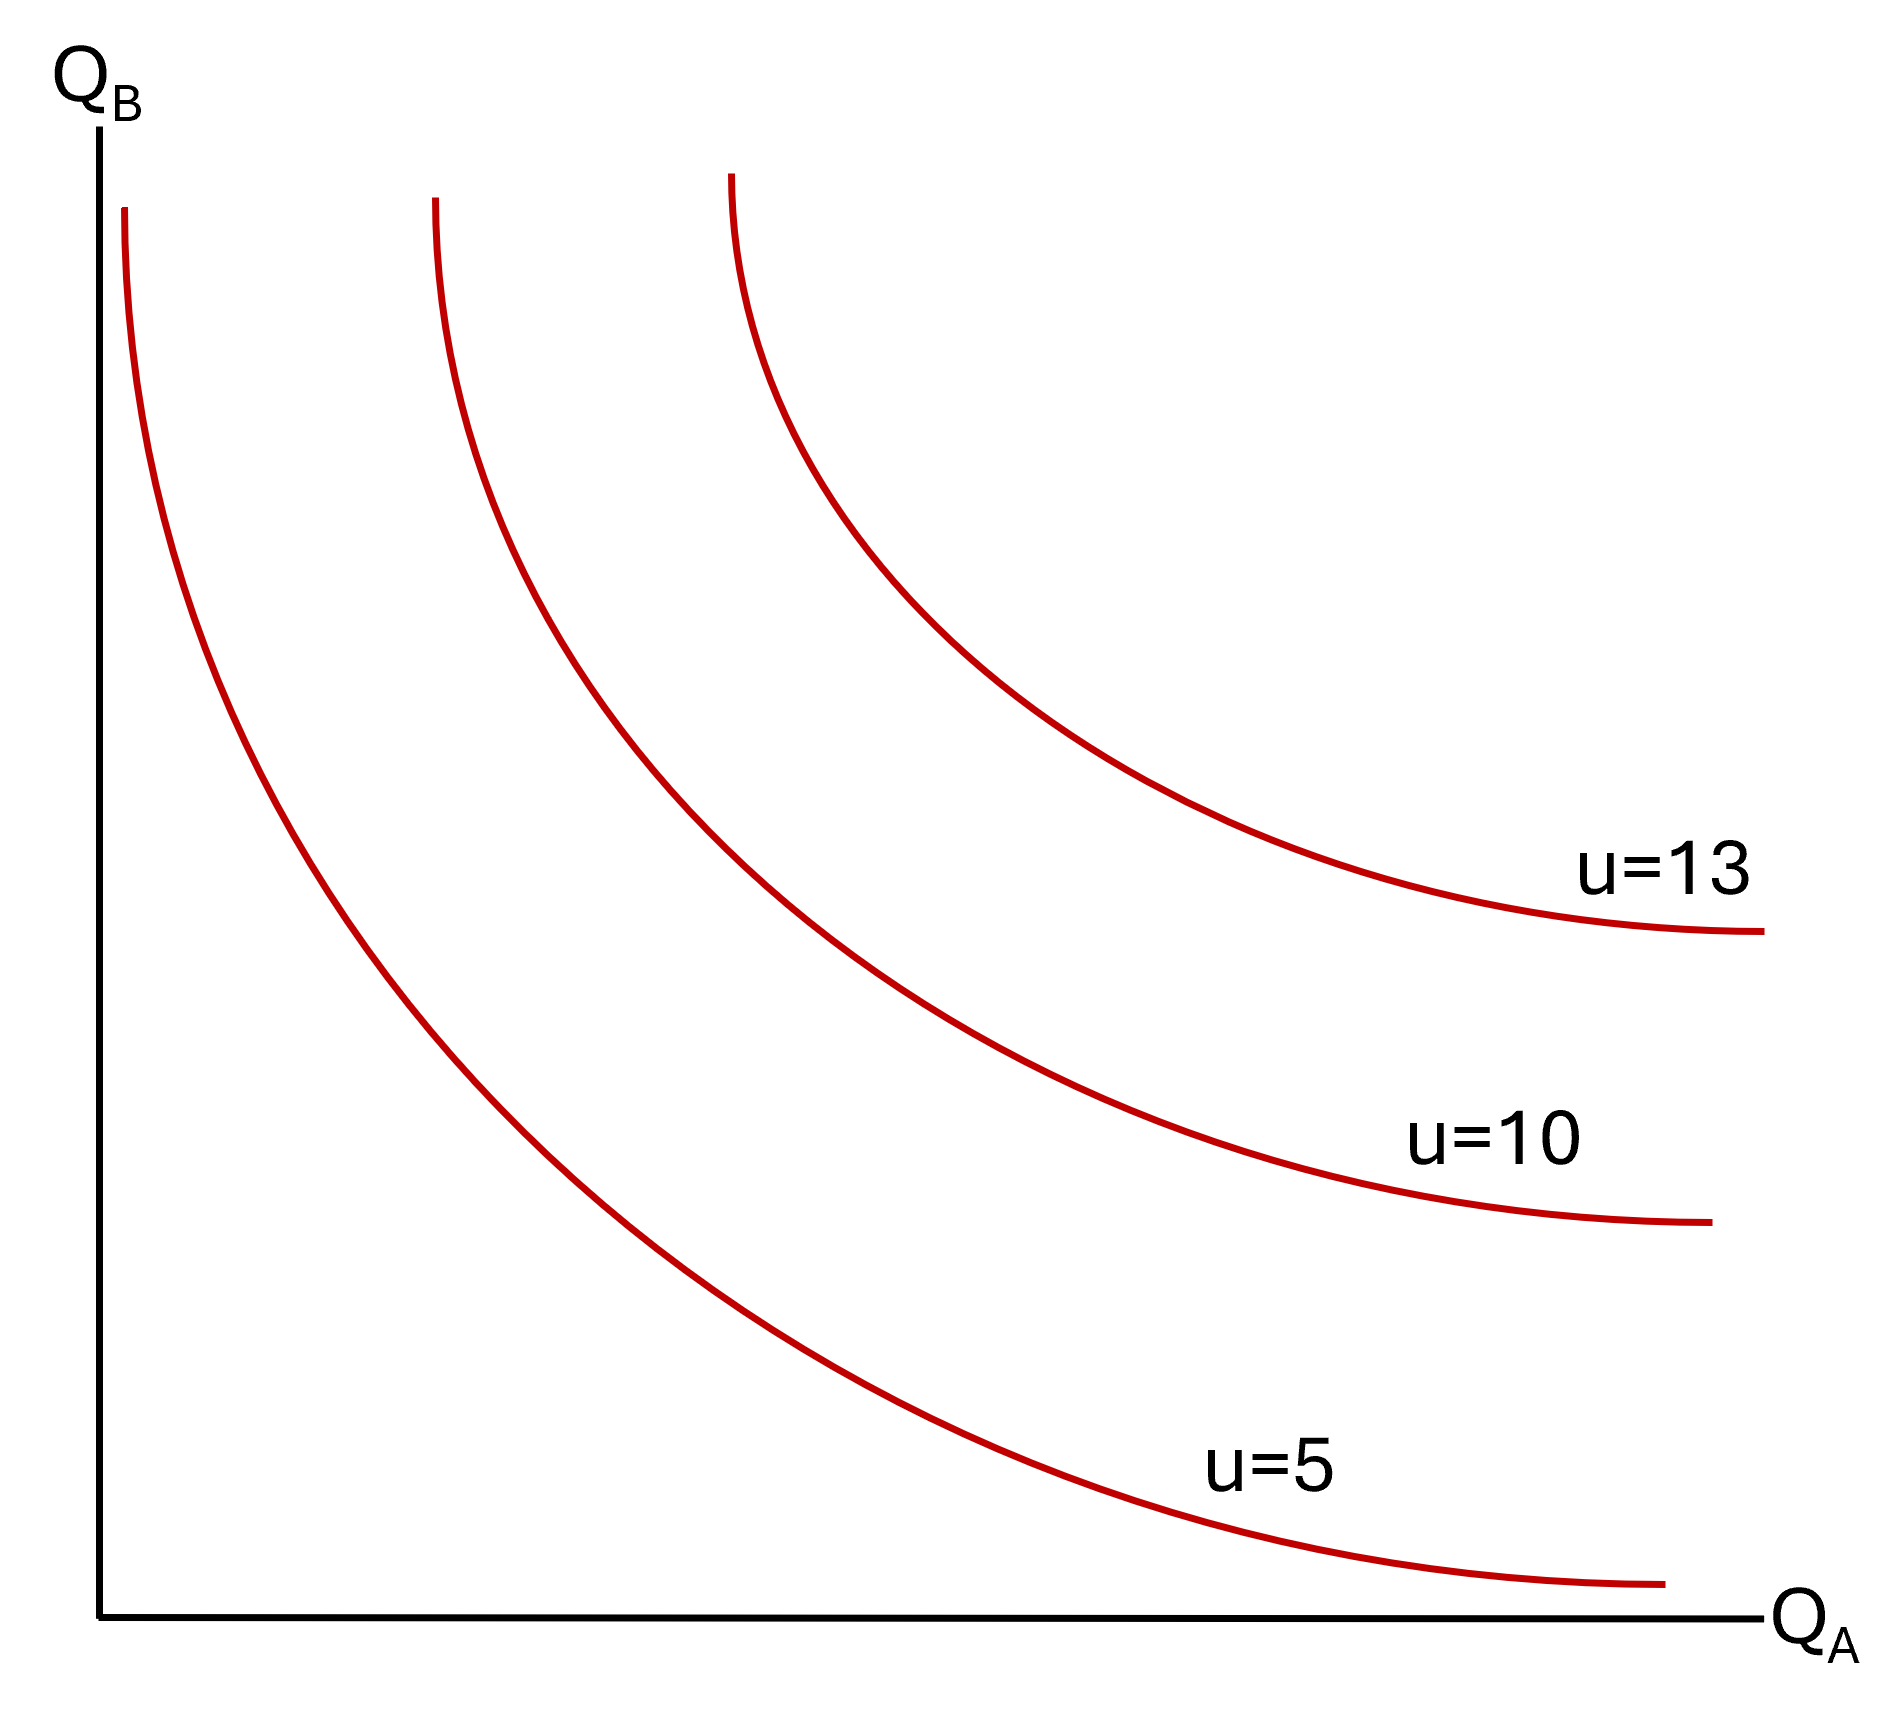
\includegraphics[width=0.5\linewidth]{indifference_curves.png}
    \end{figure}
\end{frame}

\begin{frame}{Marginal Rate of Substitution}
    \begin{itemize}
        \item MRS:  How much $B$ I'm willing to give up for one unit of $A$.
        \item Just the negative slope of the indifference curve between two points:\\$MRS = -(B_1 - B_2)/(A_1 - A_2)$
    \end{itemize}
    \centering
    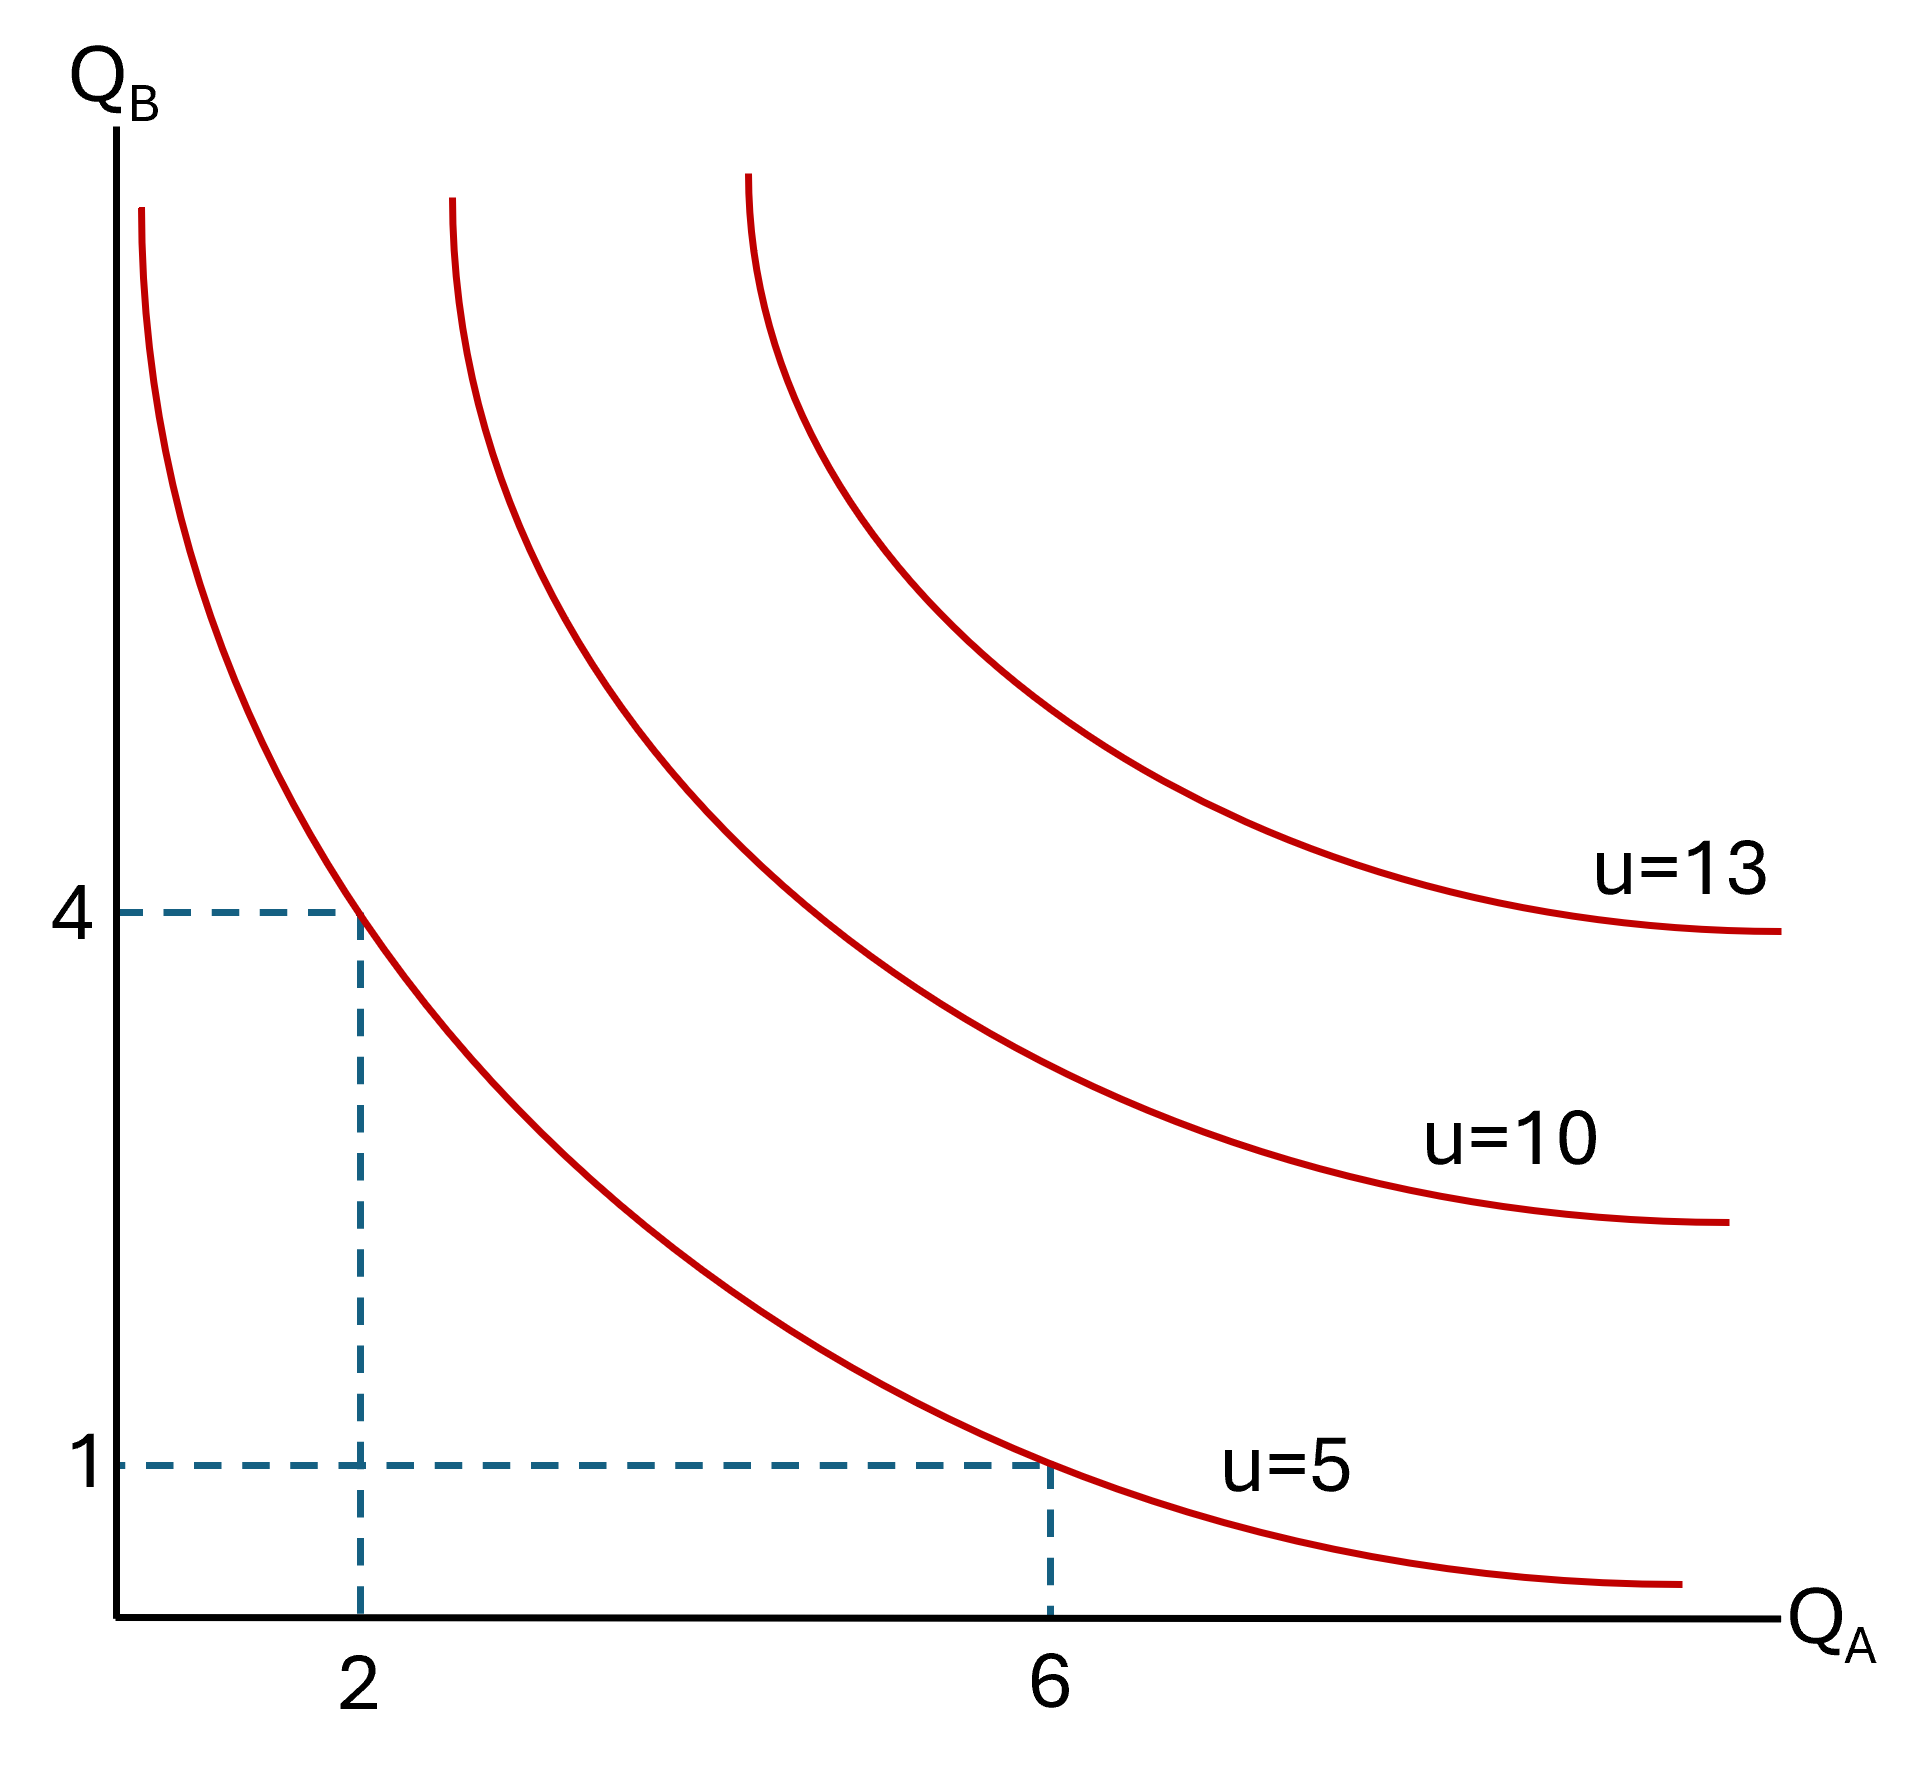
\includegraphics[width=0.5\linewidth]{mrs.png}
    \begin{itemize}
        \item In this case, $MRS = 3/4$.  ``I can give up 3/4 bananas for 1 apple and be indifferent".
    \end{itemize}
\end{frame}

\begin{frame}{Optimal Consumption Point}
    \begin{itemize}
        \item Consumer maximizes utility subject to budget constraint.
        \item ``Climb as high up the hill as possible" while staying behind the BC.
    \end{itemize}
    \begin{figure}
        \centering
        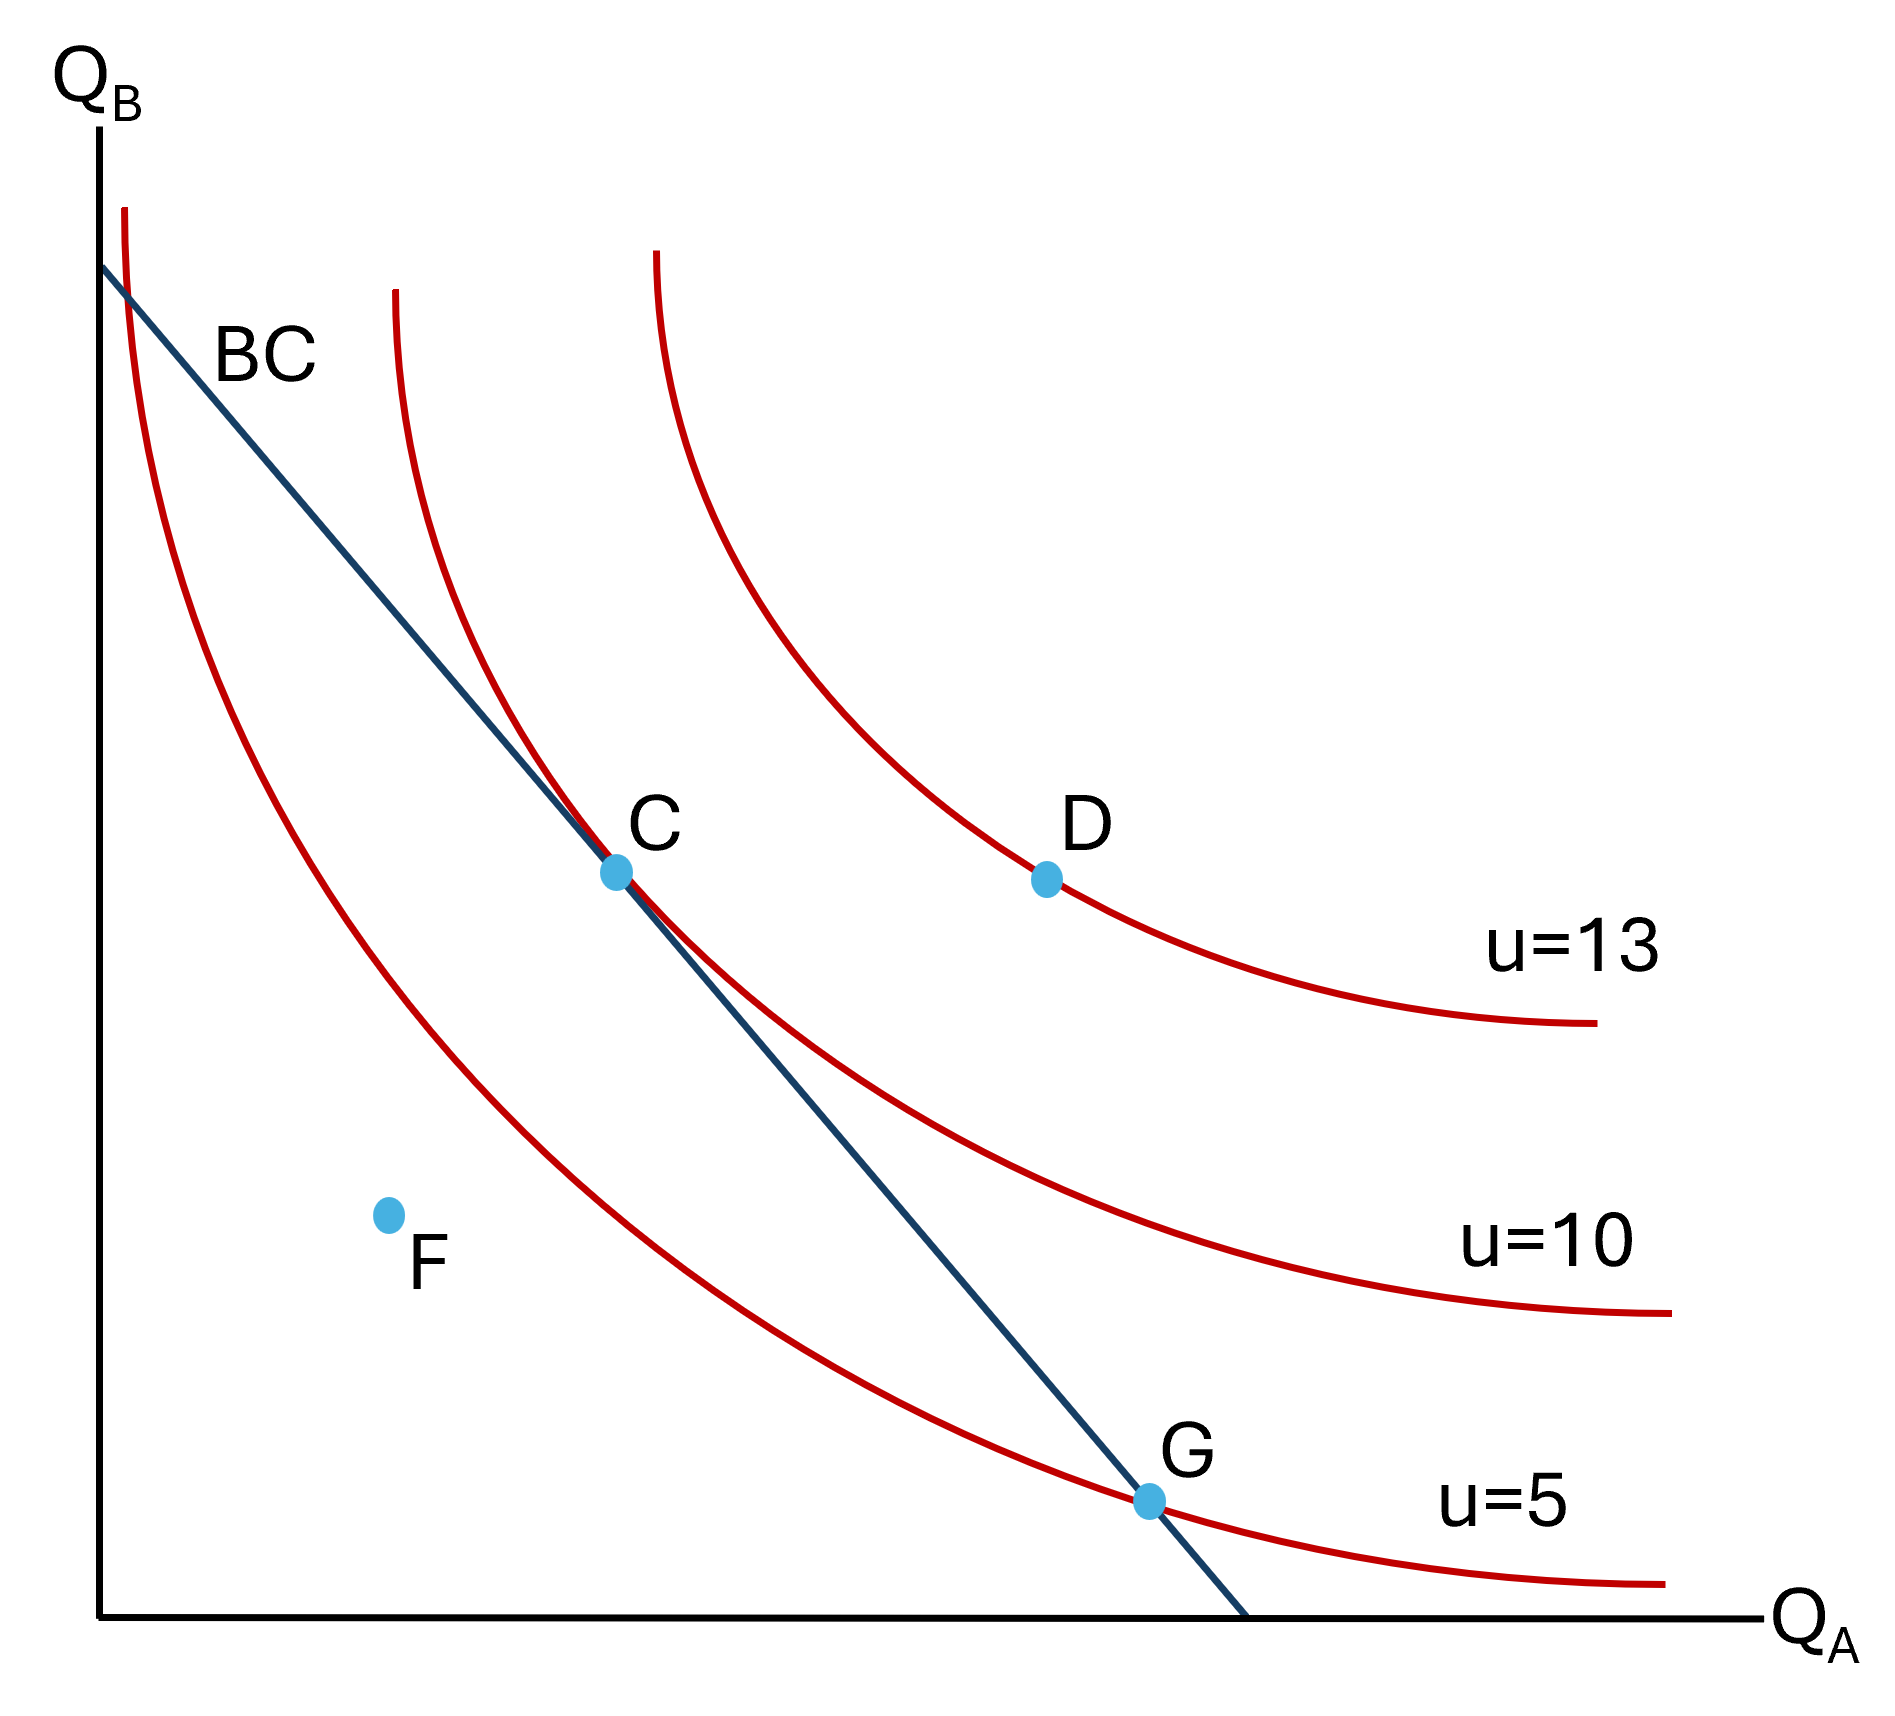
\includegraphics[width=0.5\linewidth]{optimum.png}
    \end{figure}
\end{frame}

\begin{frame}{Optimal Consumption Point}
    \begin{itemize}
        \item Consumer maximizes utility subject to budget constraint.
        \item ``Climb as high up the hill as possible" while staying behind the BC.
    \end{itemize}
    \begin{figure}
        \centering
        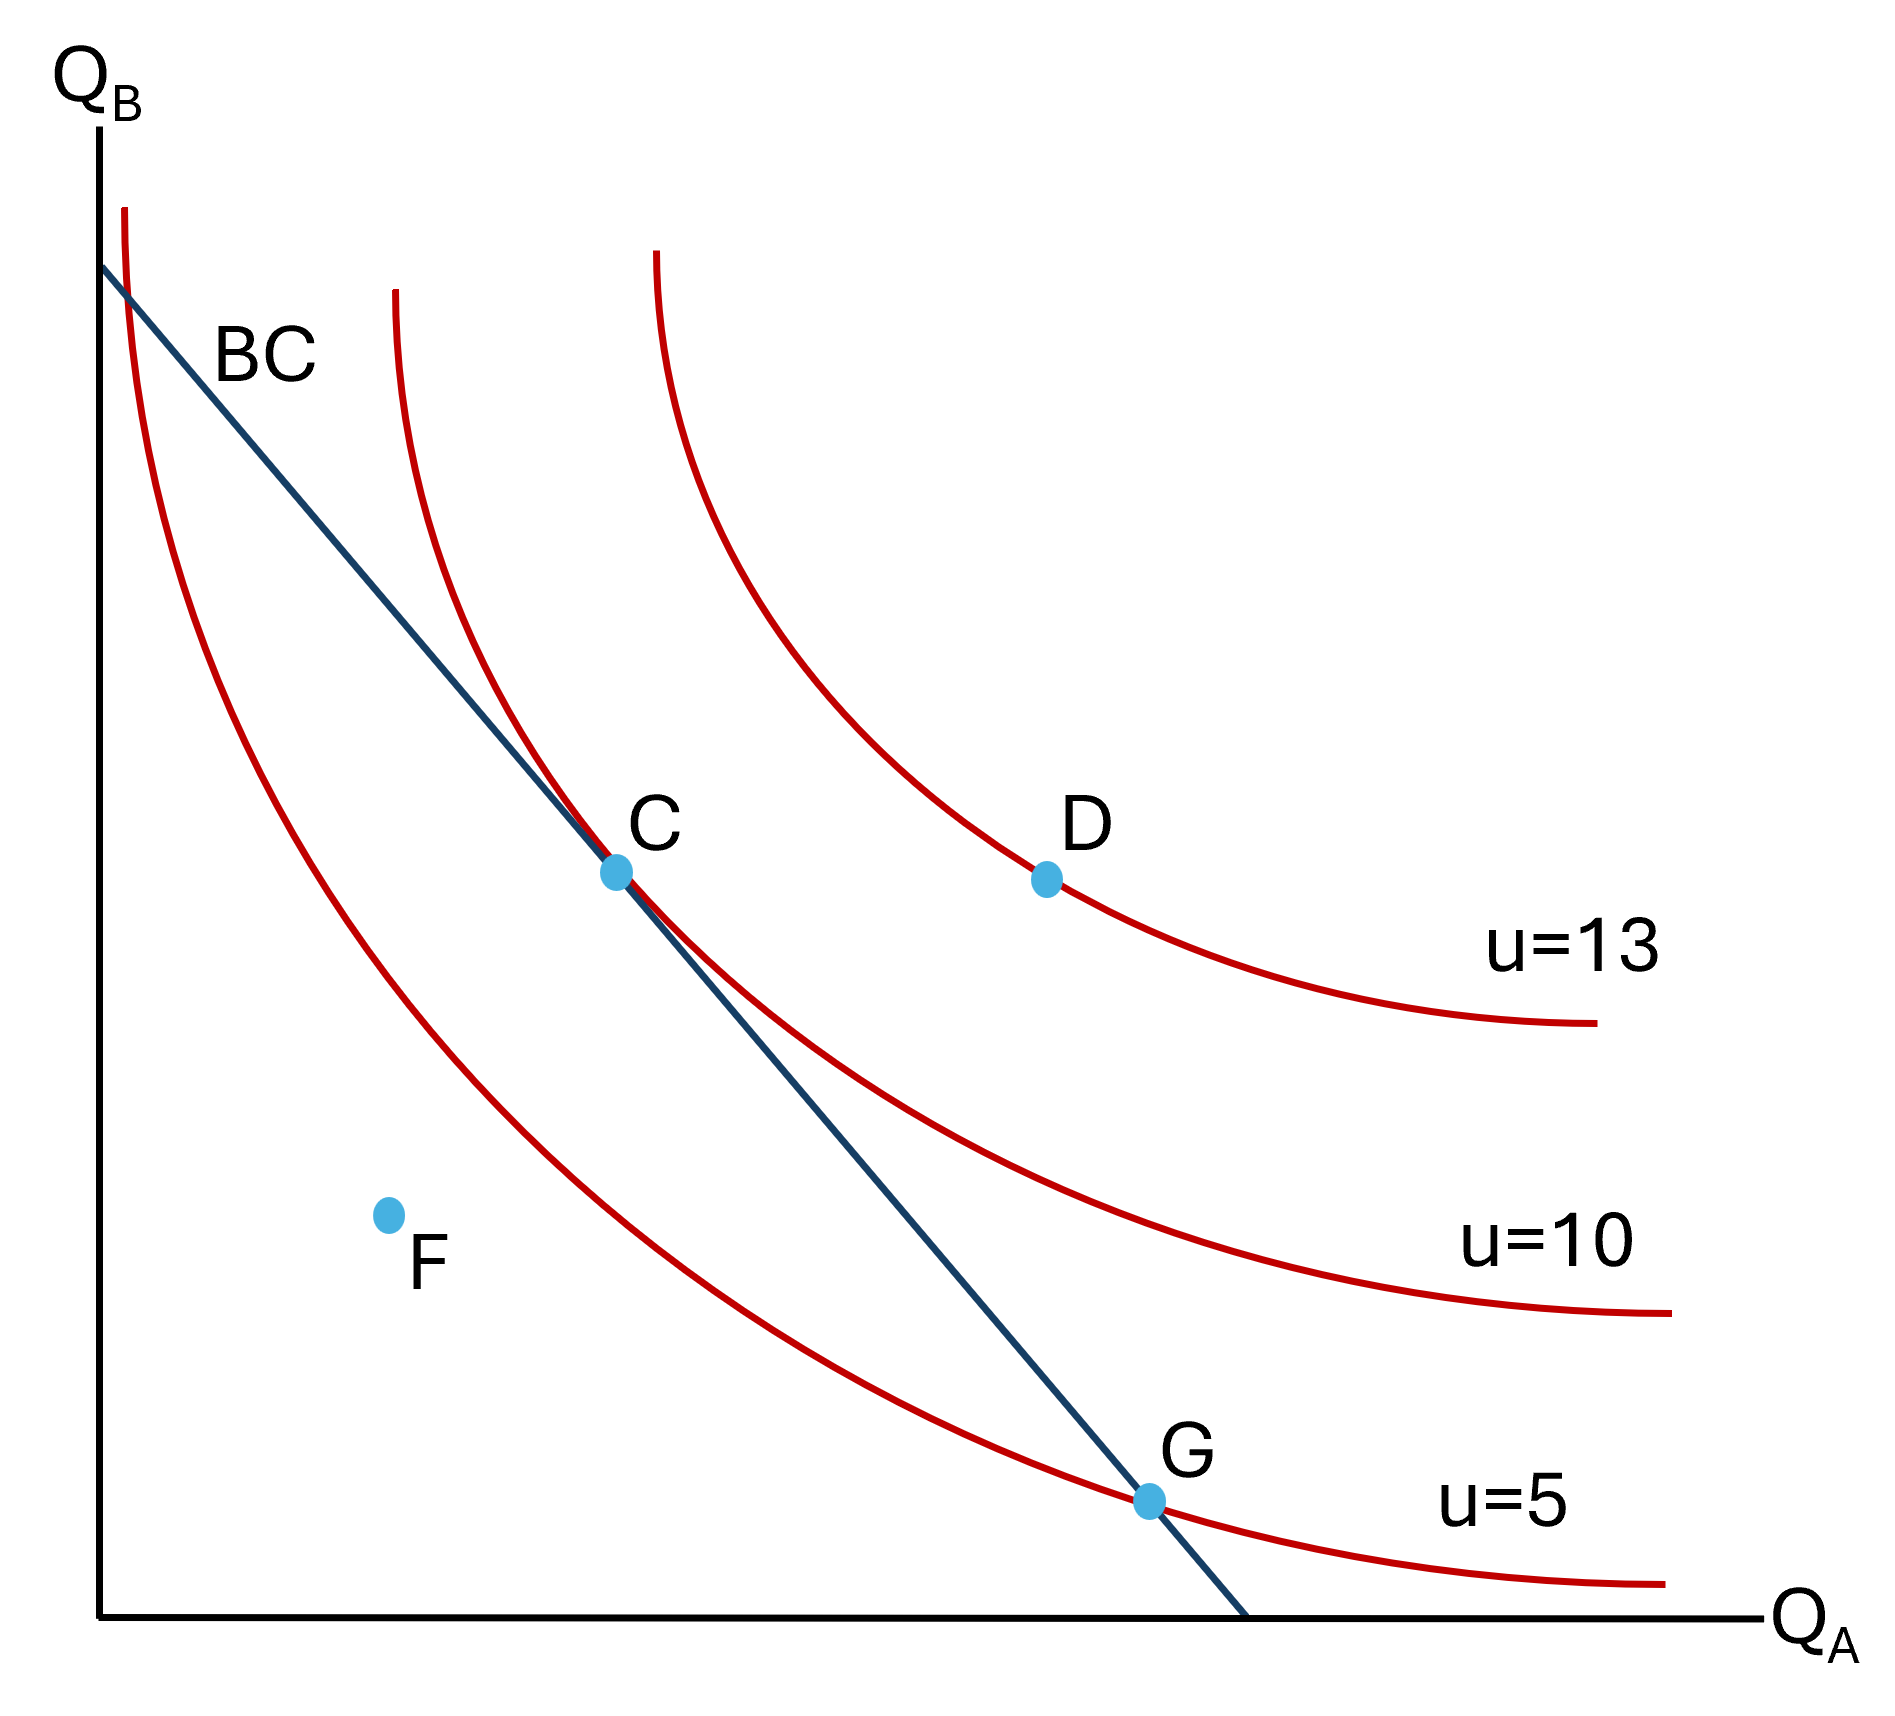
\includegraphics[width=0.5\linewidth]{optimum.png}
    \end{figure}
    \begin{itemize}
        \item<2-> At point $C$, the (negative) slope of the BC is equal to the MRS (slope of the IC)
    \end{itemize}
\end{frame}

\begin{frame}{Exercise 2: Indifference Curve \& Optimal Choice}
    Q1: Consider the following indifference curve.
    \begin{enumerate}
        \item Calculate the marginal rate of substitution (MRS) from point B to C
        \item Suppose the price of ice cream bars and strudels are both \$10. Your income is \$110. Draw and label your budget constraint and mark the optimal choice in relation to an indifference curve. 
        \item Suppose your income increases to \$220. How will your optimal choice change if 
        \begin{itemize}
            \item[-] ice cream bar is a normal good?
            \item[-] ice cream bar is an inferior good? 
        \end{itemize}
        How must your indifference curves be shaped in each of those scenarios?
    \end{enumerate}
    \begin{figure}
        \centering
        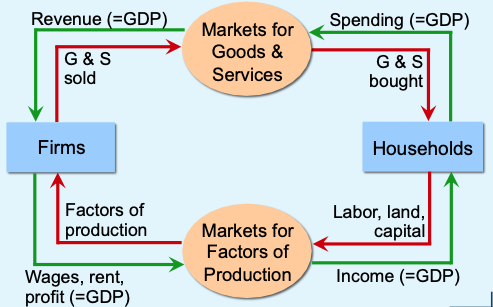
\includegraphics[width=0.4\linewidth]{fig1.jpg}
    \end{figure}
\end{frame}

\begin{frame}{Exercise 2: Indifference Curve \& Optimal Choice}
    Solution: 
    \begin{enumerate}
        \item $MRS=\frac{34-23}{11-7}=\frac{11}{4}$
        \item The optimal choice is the tangent point of the indifference curve to the budget line 
        \begin{figure}
            \centering
            \includegraphics[width=0.35\linewidth]{sol2_a.png}
        \end{figure}
        \item Changes in optimal choice: 
        \begin{figure}[h!]
            \centering
            \includegraphics[width=0.8\linewidth]{sol2_b.png}
        \end{figure}
    \end{enumerate}
\end{frame}

\begin{frame}{Externalities}
    \begin{itemize}
        \item When a market transaction effects a third party.
        \vspace{5pt}
        \item \textbf{Negative Externality:} The third party is negatively effected.
        \vspace{3pt}
        \begin{itemize}
            \item Quantity produced is too high.
            \item Policy response is a tax.
        \end{itemize}
        \vspace{5pt}
        \item \textbf{Positive Externality:} The third party is positively effected.
        \vspace{3pt}
        \begin{itemize}
            \item Quantity produced is too low.
            \item Policy response is a subsidy.
        \end{itemize}
    \end{itemize}
\end{frame}

\begin{frame}{Exercise 3: Externalities}
    Q1: Consider the following market for beers:
    \begin{itemize}
        \item[-] $Q^D = 20 - P$
        \item[-] $Q^S = P - 2$
    \end{itemize}
    Suppose that drinking beers at a party makes the party more fun for everybody, including non-drinkers, to the tune of \$2 of fun per beer.
    \vspace{5pt}
    \begin{enumerate}
        \item Find the market equilibrium quantity.
        \item What kind of externality is this?
        \item What is the appropriate policy response?
        \item How big should the response be? 
        \item Assume the policy is implemented. Find the socially optimal quantity.
    \end{enumerate}
    \vspace{1in}
\end{frame}

\begin{frame}{Exercise 3: Externalities}
    Solution:
    \begin{enumerate}
        \item $P=11, \: Q = 9$
        \item Positive
        \item Beer should be subsidized
        \item The size of the externality: $\sigma = \$2$
        \item $P^D = P^S - 2 \:$, so 
    \end{enumerate}
    \begin{align*}
        Q^D(P^D) &= Q^S(P^S)\\
        20 - P^D &= P^S - 2\\
        20 - (P^S - 2) &= P^S - 2\\
        \implies \: P^S &= 12,\\
        P^D &= 10,\\
        Q^{\textrm{optimal}} &= 10.
    \end{align*}
\end{frame}


\end{document}
